\clearpage 
\section{Studies on the excess observed in \ttbar\ + $X$ validation regions}
[NOTE: These results are obtained with the the old (mc15) \ttbar~+~$V$ samples, and are not updated with the mc15b samples, latest cross-sections and k-factors.]
\label{appendix:ttV}

In this appendix we summarize the studies performed to understand the excess observed in the \ttbar~+~$Z$ and \ttbar~+~$V$ validation regions. Results are obtained with 3.2~\ifb of data and using the latest recommendations.

In the tables presenting the results, the systematic uncertainty assigned to the fake lepton estimation is obtained using the ``conservative'' approach (i.e it can be reduced up to a factor 2). To account for this and for the missing sources of systematics (i.e JES, JER, etc) the discovery significance is computed using {\tt RooStats::NumberCountingUtils::BinominalObsZ} function with background uncertainty set to stat + 50\% syst. 
 
 %%%%%
\par{\bf Results in \ttbar\ + $Z$ validation regions\\}
In Table~\ref{tab:ttZ_VR_app} we recall the definition of the \ttbar\ + $Z$ validation region ($ttZ$ 1bIncl), which is a combination of 1$b$-jet exclusive ($ttZ$ 1bExcl) and 2$b$-jet inclusive ($ttZ$ 2bIncl) regions. For completeness, the results obtained in the three regions are presented in Table~\ref{tab:ttz_results} (combined channels) and in Table~\ref{tab:ttz_results_perCh} (per channel). The discovery significance of the excess in the combined channel is 0.79$\sigma$. Figure~\ref{fig:Results_VRttZ_ttV} (top and bottom-left) presents the \meff\ distribution in these regions. It can be noticed that the excess tends to be more in the low \meff\ region ($<$~500~\GeV). Looking separately at the $ttZ$ 1bExcl and $ttZ$ 2bIncl regions it is clear that the excess is driven by the latter region selection. The discovery significance in this region is 2.08$\sigma$. 

\begin{table}[htb!]
\begin{center}
 \resizebox{\textwidth}{!}{
    \begin{tabular}{|c|c|c|c|}
      \hline 
      \hline
      VR& $ N_{lept}^{signal}$ & $N_{b-jets}^{20}$   & Other variables \\ \hline
    $ttZ$ 1bExcl & $\ge$3, \pt : (l1, l2, e3 ($\mu3$)) = (25, 25, 20 (10)) GeV & ==1  & 20 $<$ \met $<$ 150 \GeV, 100 $<$ \meff $<$ 900 \GeV,  \\
   &  & & $N_{jets}^{25}$ $\ge$ 4, $|\eta|_{e1,2}$~$<$~1.37, $80 < m^{SFOS}_{\ell\ell} < 100$~GeV, !SR\\\hline
    $ttZ$ 2bIncl& $\ge$3, \pt : (l1, l2, e3 ($\mu3$)) = (25, 25, 20 (10)) GeV & $\ge$2  & 20 $<$ \met $<$ 150 \GeV, 100 $<$ \meff $<$ 900 \GeV, \\
   &  & & $N_{jets}^{25}$ $\ge$ 3, $|\eta|_{e1,2}$~$<$~1.37, $80 < m^{SFOS}_{\ell\ell} < 100$~GeV, !SR\\\hline
\end{tabular}}
\end{center} 
\vspace{-0.5cm}
\caption{\ttbar\ + $Z$ validation region definition ($ttZ$ 1bIncl = $ttZ$ 1bExcl || $ttZ$ 2bIncl).}
\label{tab:ttZ_VR_app}
\end{table}
%%
\begin{table}[htb!]
\begin{center}
\resizebox{\textwidth}{!}{
    \begin{tabular}{|c|c|c|c|}
      \hline 
      \hline
     VR& $ N_{lept}^{signal}$ & $N_{b-jets}^{20}$     & Other variables \\ \hline
    $ttV$ 2bIncl& $\ge 2$, \pt : (l1, l2, l3) = (25, 25, 10) GeV & $\ge$2  & 20 $<$ \met $<$ 200 \GeV, 200 $<$ \meff $<$ 900 \GeV, $|\eta|_{e1,2}$~$<$~1.37, \\
   &  && $N_{jets}^{25}$ $\ge$ 5 in $ee$ and $e\mu$, $N_{jets}^{25}$ $\ge$ 3 in $\mu\mu$ channels, !SR\\\hline
\end{tabular}}
\end{center}
\vspace{-0.5cm}
\caption{\ttbar\ + $V$ validation region definition ($ttV$ 2bIncl). }
\label{tab:ttV_VR_app}
\end{table}


\begin{table}[htb!]
\begin{center}
\begin{tabular}{|c|ccc|}
\hline\hline
 & $ttZ$ 1bIncl &  $ttZ$ 1bExcl &$ttZ$ 2bIncl\\\hline
          Fakes &  $0.65 \pm 0.60 \pm 1.88$ & $0.90 \pm 0.41 \pm 0.74$ &$-0.25 \pm 0.43 \pm 1.13$ \\
            ttZ  & $4.38 \pm 0.08 \pm 1.31$ & $1.85 \pm 0.05 \pm 0.56$& $2.52 \pm 0.06 \pm 0.76$ \\
            ttW  & $0.09 \pm 0.02 \pm 0.03$ & $0.02 \pm 0.01 \pm 0.01$& $0.08 \pm 0.02 \pm 0.02$ \\\hline
            Total  & $7.74 \pm 0.65 \pm 3.00$ & $4.42 \pm 0.46 \pm 1.36$& $3.32 \pm 0.46 \pm 1.65$ \\ 
           Data  & $14  $ & $2 $ & $12  $ \\ \hline \hline
           Significance & 0.79 & -1.35 & 2.08 \\ \hline
\end{tabular}
\end{center}
\vspace{-0.5cm}
\caption{Results in $ttZ$ 1bExcl, $ttZ$ 1bIncl and $ttZ$ 2bIncl regions. All channels are combined. ``Total'' includes the number of expected background events.}
\label{tab:ttz_results}
\end{table}
%%
\begin{table}[htb!] 
\begin{center}
\resizebox{0.7\textwidth}{!}{
\begin{tabular}{|c|ccc|}
\hline\hline
 & $ttZ$ 1bIncl & $ttZ$ 1bExcl &  $ttZ$ 2bIncl\\\hline
\hline\multicolumn{4}{c}{\bf $ee$ channel}\\\hline
          Fakes & $-0.44 \pm 0.24 \pm 0.36$  & $-0.02 \pm 0.02 \pm 0.03$& $-0.42 \pm 0.24 \pm 0.33$ \\
           ttZ & $0.56 \pm 0.03 \pm 0.17$ & $0.24 \pm 0.02 \pm 0.07$ & $0.33 \pm 0.02 \pm 0.10$ \\
            ttW  & $0.02 \pm 0.01 \pm 0.00$ & $0.00 \pm 0.00 \pm 0.00$& $0.02 \pm 0.01 \pm 0.00$ \\\hline
            Total  & $0.42 \pm 0.26 \pm 0.46$ & $0.38 \pm 0.07 \pm 0.13$& $0.05 \pm 0.25 \pm 0.36$ \\
           Data& $3 $  & $0  $ & $3  $ \\
           Significance & 1.65 & - & 0.90 \\
\hline\multicolumn{4}{c}{\bf $e\mu$ channel}\\\hline
          Fakes  & $0.62 \pm 0.40 \pm 0.76$& $0.54 \pm 0.32 \pm 0.37$ & $0.09 \pm 0.24 \pm 0.39$ \\
            ttZ  & $2.06 \pm 0.06 \pm 0.62$& $0.87 \pm 0.04 \pm 0.26$ & $1.19 \pm 0.04 \pm 0.36$ \\
            ttW  & $0.04 \pm 0.01 \pm 0.01$ & $0.00 \pm 0.00 \pm 0.00$& $0.04 \pm 0.01 \pm 0.01$ \\\hline
              Total  & $3.72 \pm 0.43 \pm 1.27$ & $2.05 \pm 0.35 \pm 0.61$& $1.67 \pm 0.25 \pm 0.65$ \\
           Data & $4 $& $0 $  & $4 $ \\
           Significance & -0.25 & - &0.87 \\ 
\hline\multicolumn{4}{c}{\bf $\mu\mu$ channel}\\\hline
          Fakes & $0.46 \pm 0.37 \pm 0.76$& $0.38 \pm 0.25 \pm 0.34$  & $0.08 \pm 0.27 \pm 0.41$ \\
      ttZ & $1.75 \pm 0.05 \pm 0.53$ & $0.75 \pm 0.03 \pm 0.22$ & $1.00 \pm 0.04 \pm 0.30$ \\
            ttW & $0.03 \pm 0.01 \pm 0.01$ & $0.01 \pm 0.01 \pm 0.00$ & $0.02 \pm 0.01 \pm 0.01$ \\\hline
            Total  & $3.60 \pm 0.42 \pm 1.30$ & $1.99 \pm 0.29 \pm 0.63$& $1.60 \pm 0.30 \pm 0.67$ \\
           Data & $7  $  & $2 $ & $5  $ \\
           Significance & 0.76 & -0.39 & 1.33 \\\hline
\end{tabular}}
\end{center}
\vspace{-0.5cm}
\caption{Results per channel in $ttZ$ 1bExcl, $ttZ$ 1bIncl and $ttZ$ 2bIncl regions. ``Total'' includes the number of expected background events.}
\label{tab:ttz_results_perCh}
\end{table}
%%


\begin{figure}[h!]
\centering
\subfigure{
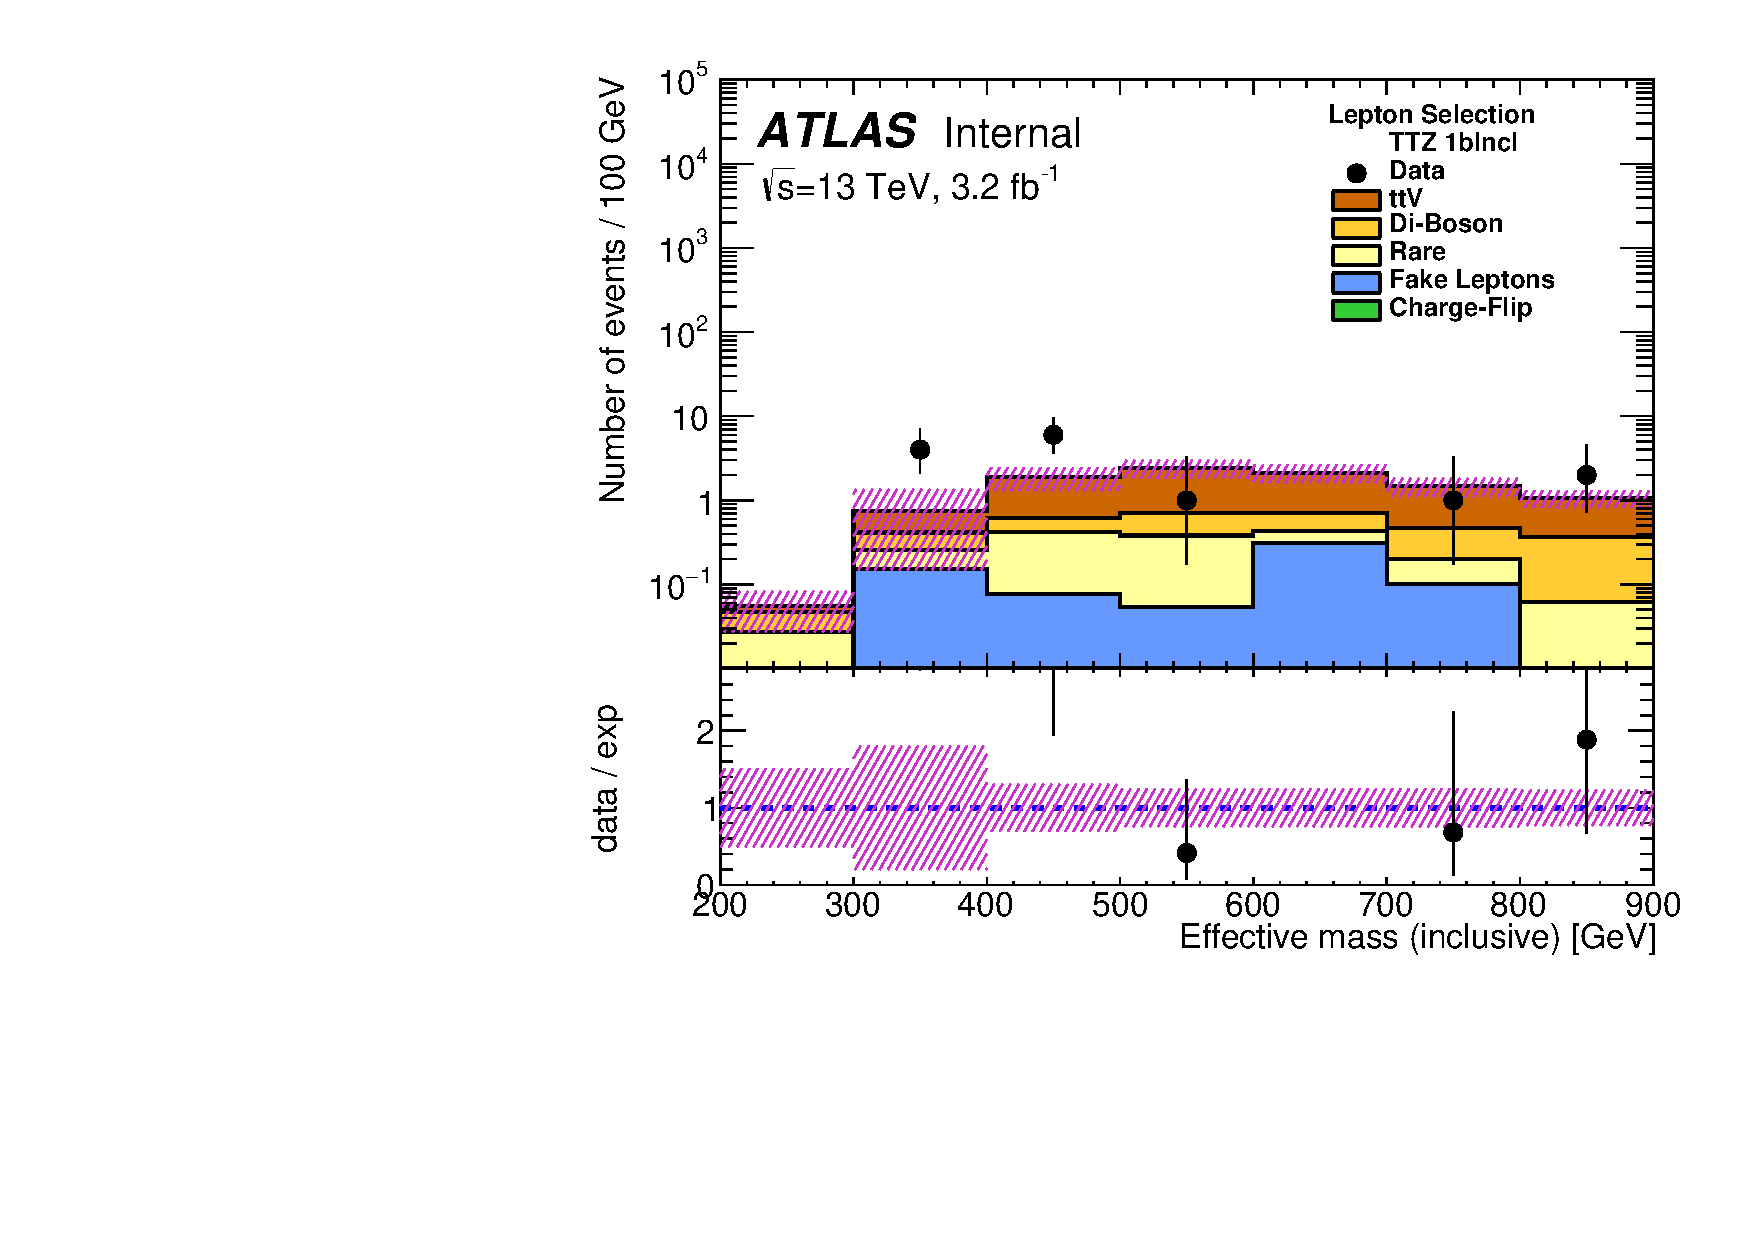
\includegraphics[width=0.45\textwidth]{BKG/validationPLots/TTZ_CR1bIncl_MEFF}
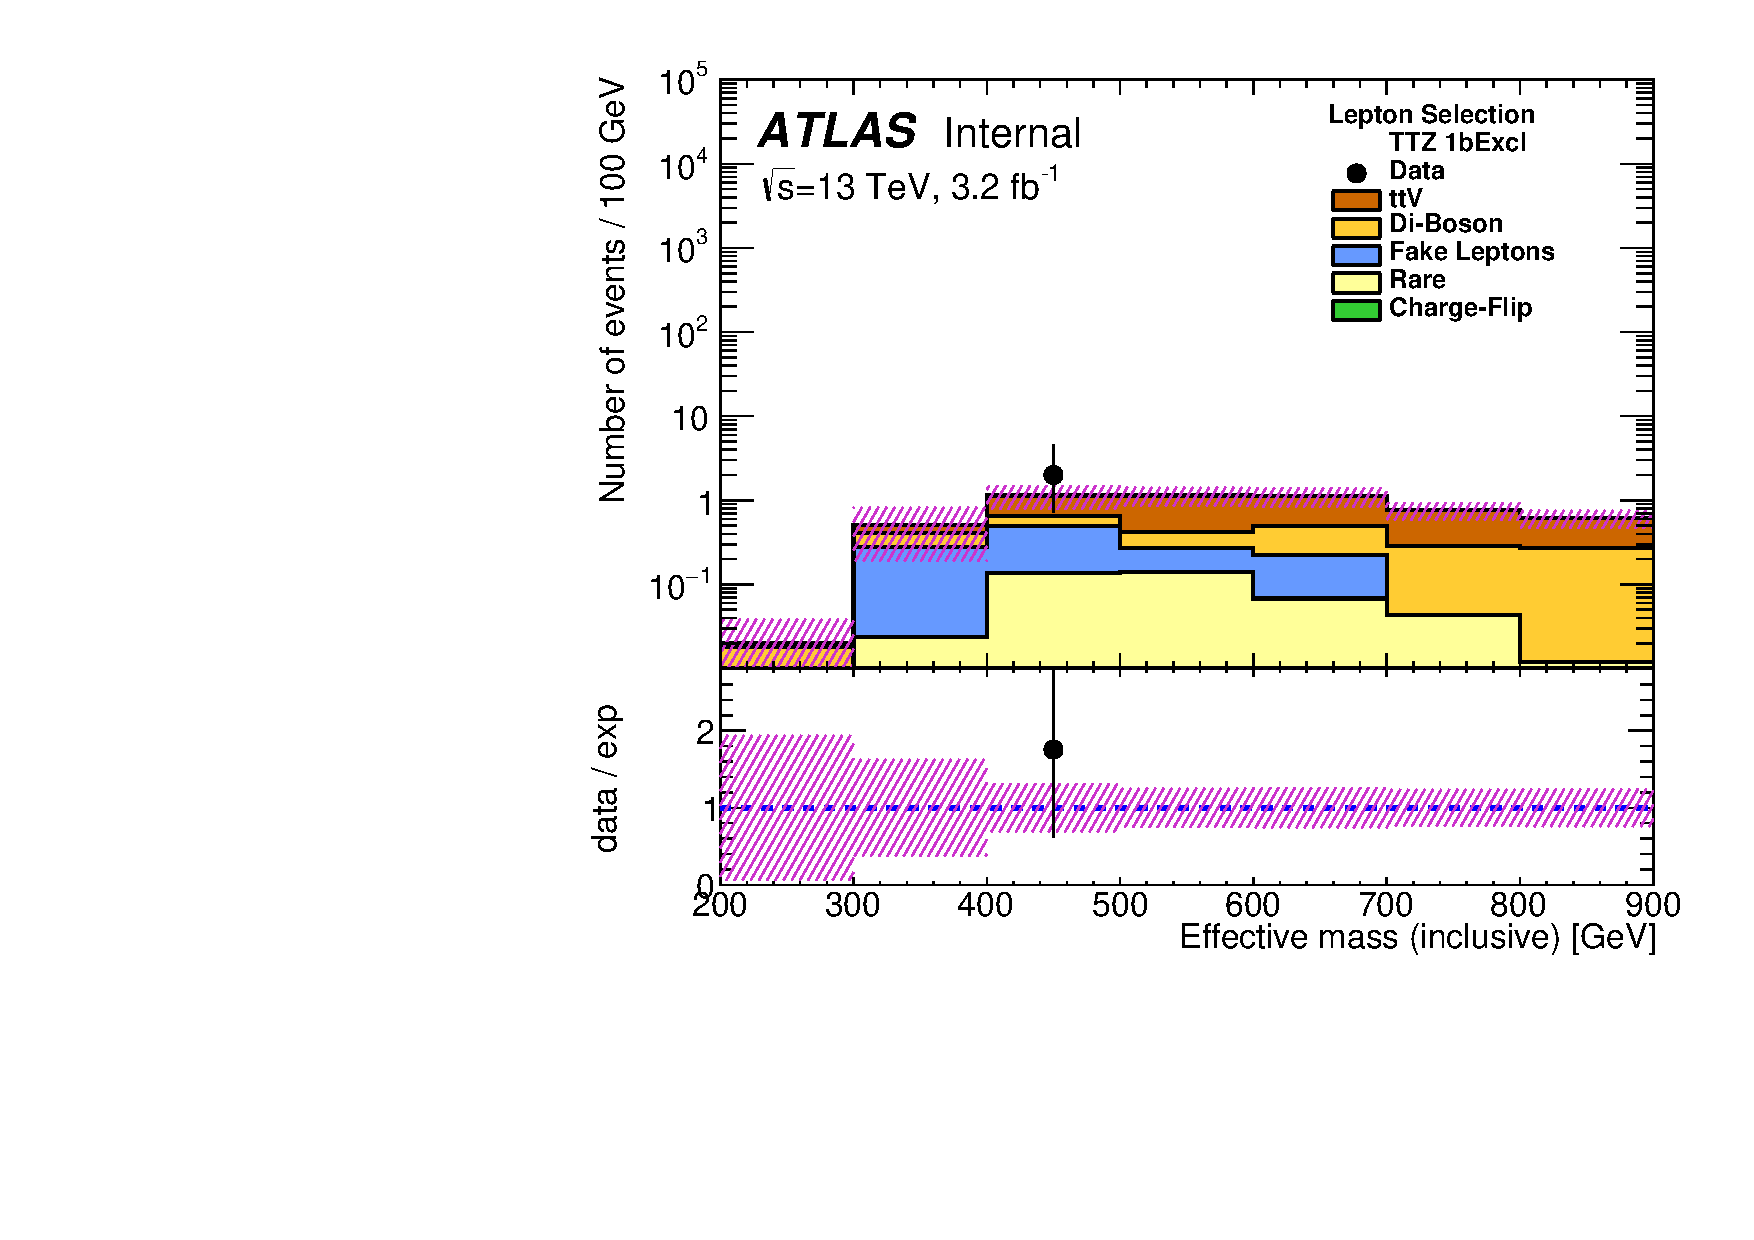
\includegraphics[width=0.45\textwidth]{BKG/validationPLots/TTZ_CR1bExcl_MEFF}}
\subfigure{
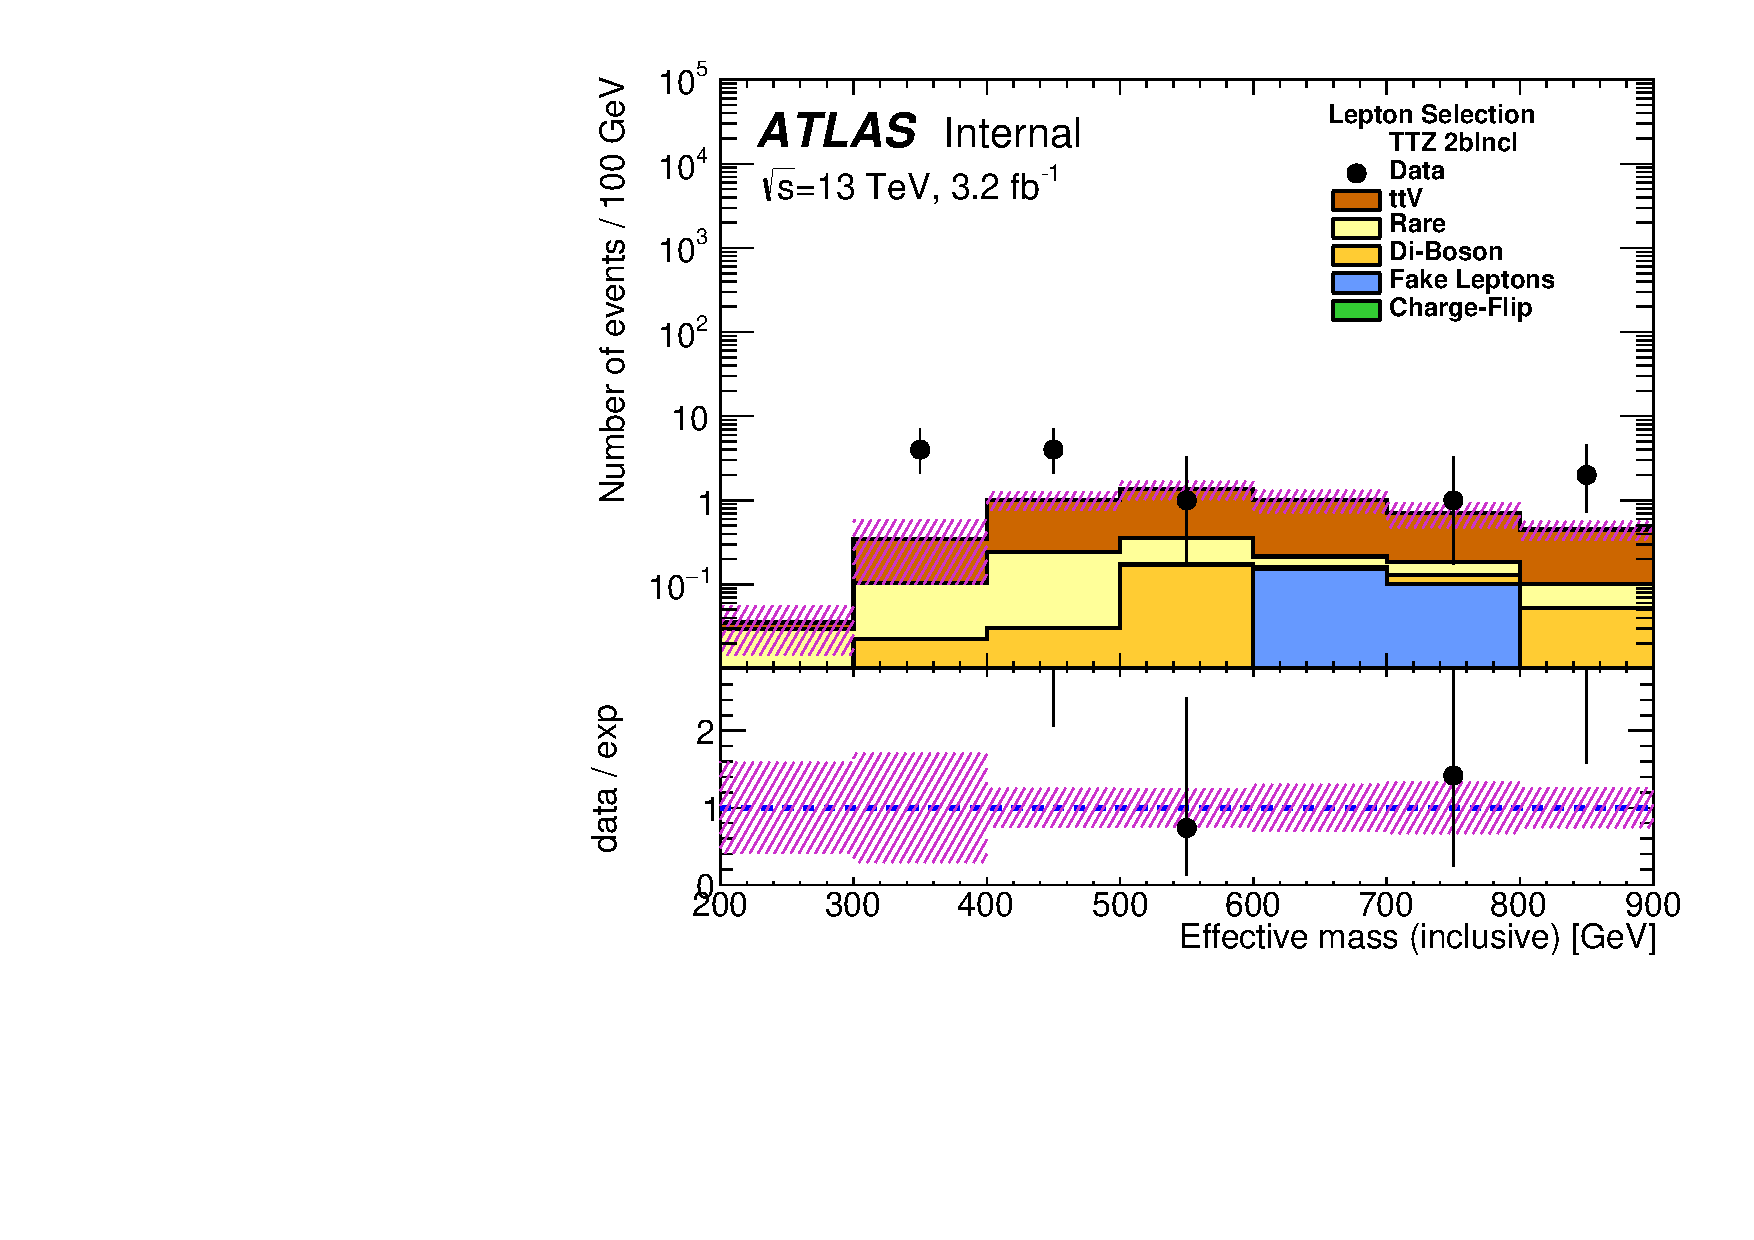
\includegraphics[width=0.45\textwidth]{BKG/validationPLots/TTZ_CR2bIncl_MEFF}
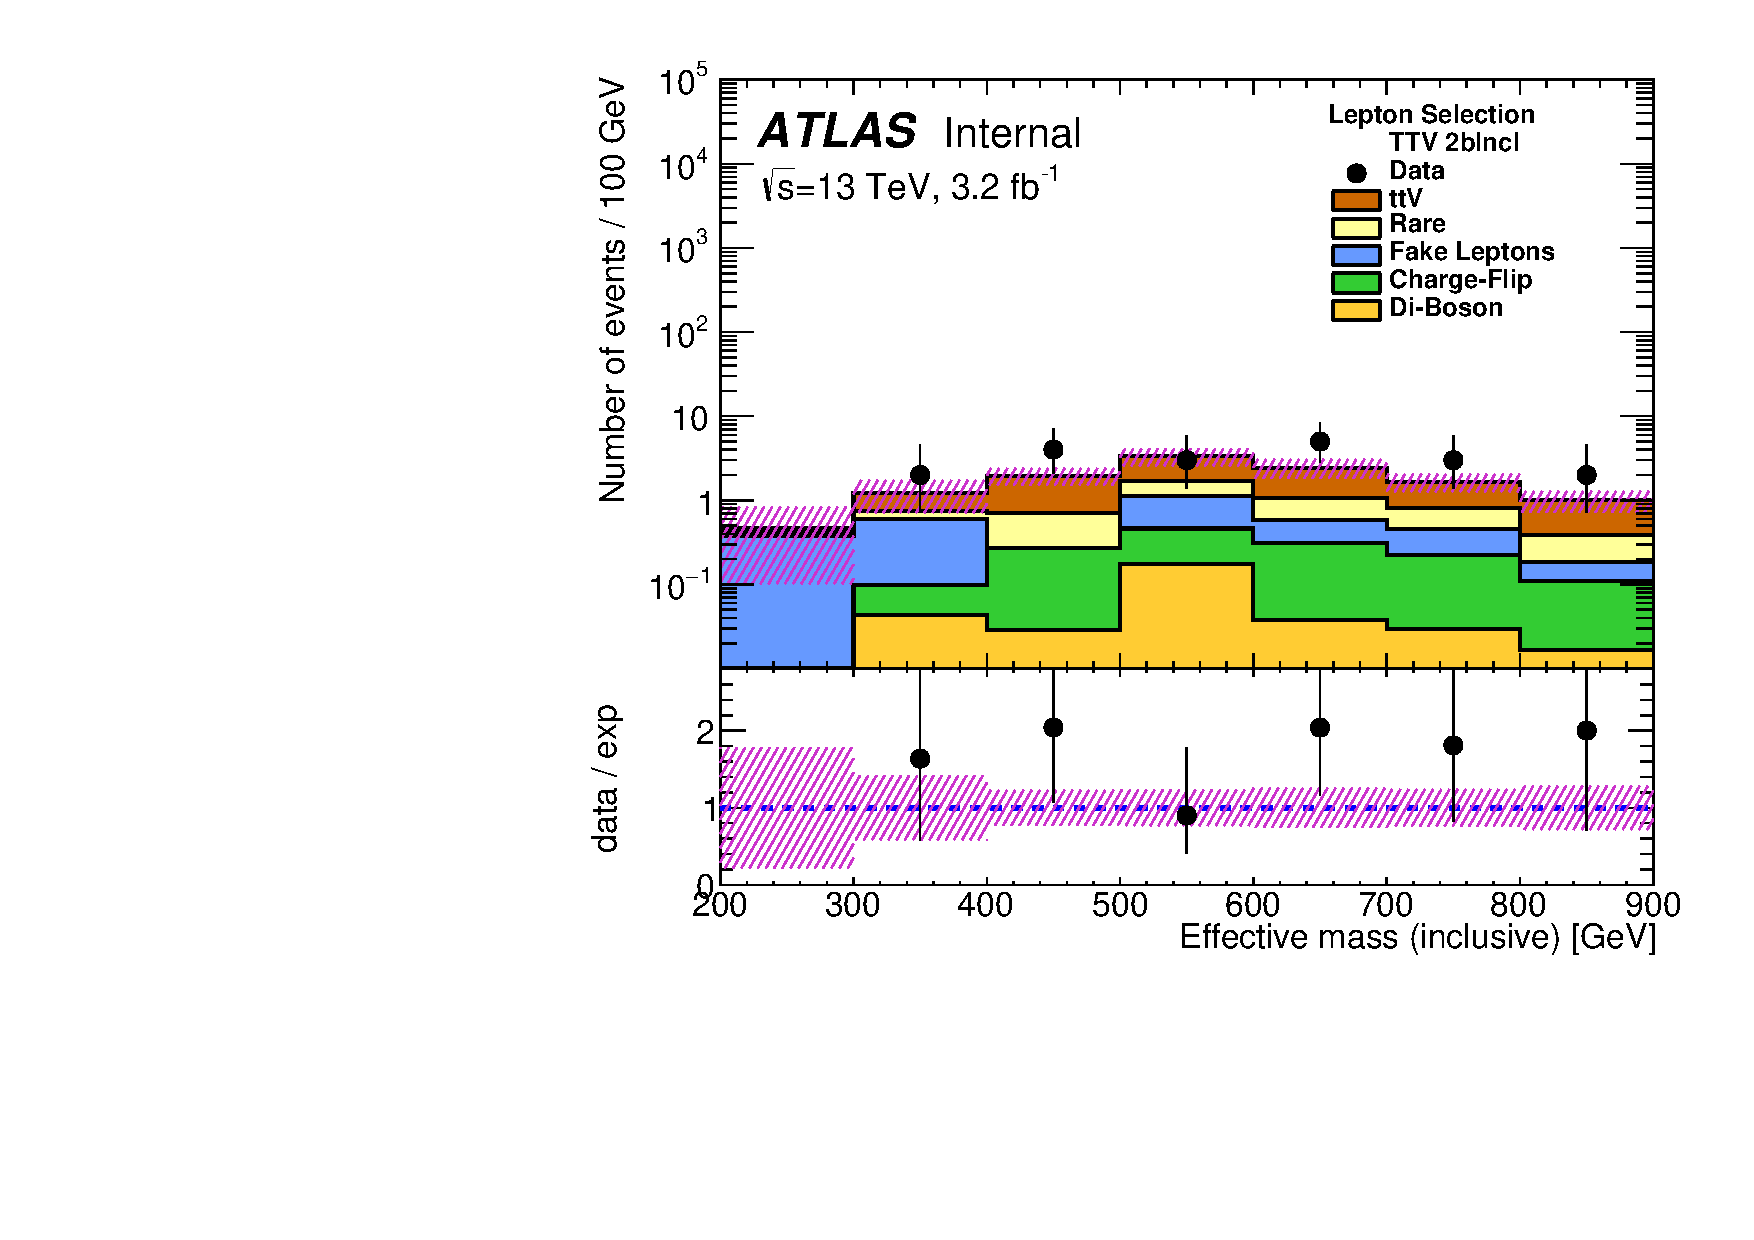
\includegraphics[width=0.45\textwidth]{BKG/validationPLots/TTV_CR2bIncl_MEFF}
}
\caption{Effective mass distribution in $ttZ$ 1bIncl (top-left), $ttZ$ 1bExcl (top-left), $ttZ$ 2bIncl (top-right) and $ttV$ 2bIncl regions.}
\label{fig:Results_VRttZ_ttV}
\end{figure}
  
 
 %%%%%
\par{\bf Candidates in $ttZ$ 1bIncl \\}
The observed events in data are shown in Table~\ref{table:Candidates_ttZ}. It can be seen that all leptons are well isolated and most of the leading leptons have a transverse momentum higher than 70-100~\GeV. Such properties reduce the chance to have a hight amount of fake leptons. In this validation region only two events have 3 $b$-jets and 0 events have $\geq$4 $b$-jets; only two events have 4 leptons. 

In Table~\ref{table:Candidates_ttZ_ttV_common} are shown the candidates common in $ttZ$ and $ttV$ 2bIncl regions. It helps to understand if the excess present in the latter region is found back in the $ttZ$ 2bIncl VR. A total of 8 events out of 12 are found to be in both regions; the other 4 events are not passing the number of jets cut ($\geq$5 in the $ee$ and $e\mu$ channels). In $ttV$ 2bIncl VR 19 events are observed, as shown in Tables~\ref{table:Candidates_ttZ_ttV_common} and~\ref{table:Candidates_ttV}. For illustration, Figure~\ref{fig:Results_VRttZ_ttV} (bottom) shows side by side the \meff\ distribution in these two regions. It is clear that the tension in the \meff~$<$~500~\GeV region diminishes with the selection proposed for $ttV$ 2bIncl VR (2 events are not passing the N$_{jets}^{25}$ cut). 

%
\begin{sidewaystable}[ph!]
\centering
\renewcommand{\arraystretch}{1.2}
{
\resizebox{1.\textwidth}{!}{
\begin{tabular}{|c|c|c|c|c|c|c|c|c|c|c|c|} \hline
 & Run & Event Number & nLep & Leptons ($\pt$ [GeV]) &  Leptons ($\eta$) & Leptons (rel trackIso) & Leptons (rel calo20Iso) & $\met$ [GeV] & $m_{eff}$ [GeV] & $N_{jets}^{25}$ & $N_{b-jets}^{20}$ \\ \hline  \hline
1  & 276329 & 224346343 & 3 & $\mu-$(81.71) $\mu+$(71.22) $\mu+$(24.17) & $\mu-$(1.71) $\mu+$(0.97) $\mu+$(2.12) & $\mu-$(0.00) $\mu+$(0.00) $\mu+$(0.00) & $\mu-$(0.00) $\mu+$(-0.00) $\mu+$(0.02) & 60.07 & 453.14 & 4 & 1 \\ \hline
2  & 279279 & 441589615 & 3 & $\mu+$(79.91) $\mu-$(67.23) $\mu-$(19.89) & $\mu+$(1.01) $\mu-$(0.14) $\mu-$(-2.05) & $\mu+$(0.02) $\mu-$(0.00) $\mu-$(0.00) & $\mu+$(0.01) $\mu-$(-0.01) $\mu-$(0.10) & 58.48 & 406.53 & 4 & 1 \\ \hline \hline
3  & 279598 & 791343322 & 3 & $e-$(287.20) $\mu+$(112.64) $e+$(103.26) & $e-$(-0.15) $\mu+$(0.37) $e+$(0.35) & $e-$(0.00) $\mu+$(0.00) $e+$(0.00) & $e-$(0.00) $\mu+$(0.00) $e+$(0.00) & 65.46 & 871.03 & 5 & 2 \\ \hline
4  & 282992 & 1402526301 & 3 & $e-$(161.82) $\mu-$(34.26) $e+$(25.24) & $e-$(-0.13) $\mu-$(1.90) $e+$(-0.05) & $e-$(0.00) $\mu-$(0.00) $e+$(0.00) & $e-$(0.01) $\mu-$(0.00) $e+$(0.01) & 40.19 & 585.40 & 4 & 2 \\ \hline \hline
5  & 280862 & 959305083 & 3 & $e+$(152.06) $e-$(61.63) $\mu+$(20.73) & $e+$(0.03) $e-$(0.73) $\mu+$(-1.51) & $e+$(0.00) $e-$(0.00) $\mu+$(0.00) & $e+$(0.02) $e-$(-0.00) $\mu+$(0.10) & 95.93 & 859.35 & 7 & 2 \\ \hline
6  & 280673 & 167470141 & 3 & $\mu+$(74.86) $e-$(26.49) $\mu-$(20.46) & $\mu+$(0.16) $e-$(0.57) $\mu-$(-1.62) & $\mu+$(0.00) $e-$(0.00) $\mu-$(0.00) & $\mu+$(-0.01) $e-$(-0.01) $\mu-$(0.01) & 97.88 & 456.95 & 4 & 2 \\ \hline
7  & 280950 & 1395868892 & 3 & $\mu+$(48.45) $\mu-$(46.46) $\mu-$(21.57) & $\mu+$(0.49) $\mu-$(-0.67) $\mu-$(-0.61) & $\mu+$(0.00) $\mu-$(0.00) $\mu-$(0.00) & $\mu+$(-0.01) $\mu-$(-0.01) $\mu-$(-0.03) & 58.37 & 353.50 & 3 & 2 \\ \hline
8  & 281411 & 1555870149 & 3 & $\mu-$(35.02) $\mu+$(27.49) $\mu+$(13.62) & $\mu-$(-0.41) $\mu+$(-0.62) $\mu+$(2.33) & $\mu-$(0.00) $\mu+$(0.04) $\mu+$(0.00) & $\mu-$(-0.01) $\mu+$(0.05) $\mu+$(-0.01) & 93.93 & 332.00 & 3 & 2 \\ \hline
9  & 284484 & 457656076 & 3 & $\mu+$(147.66) $\mu-$(54.04) $\mu-$(24.74) & $\mu+$(0.46) $\mu-$(1.49) $\mu-$(-0.19) & $\mu+$(0.00) $\mu-$(0.00) $\mu-$(0.00) & $\mu+$(-0.00) $\mu-$(-0.01) $\mu-$(-0.03) & 71.19 & 481.66 & 3 & 2 \\ \hline
10  & 284285 & 3510884870 & 3 & $e-$(36.89) $e+$(36.73) $e+$(33.93) & $e-$(1.01) $e+$(-0.95) $e+$(-0.38) & $e-$(0.00) $e+$(0.00) $e+$(0.00) & $e-$(0.02) $e+$(-0.02) $e+$(-0.00) & 32.42 & 382.72 & 3 & 2 \\ \hline
11   & 280753 & 161095358 & 4 & $\mu+$(100.64) $\mu+$(33.89) $\mu-$(24.95) $\mu-$(15.85) & $\mu+$(0.62) $\mu+$(-2.19) $\mu-$(-0.37) $\mu-$(-0.31) & $\mu+$(0.00) $\mu+$(0.00) $\mu-$(0.00)  $\mu-$(0.00) & $\mu+$(0.01) $\mu+$(-0.01) $\mu-$(-0.02) $\mu-$(-0.04) & 73.32 & 405.98 & 3 & 2 \\ \hline
12   & 280977 & 330636862 & 4 & $\mu+$(153.02) $\mu+$(107.77) $\mu-$(71.42) $e-$(47.89) & $\mu+$(0.16) $\mu+$(0.37) $\mu-$(0.48) $e-$(-0.97) & $\mu+$(0.00) $\mu+$(0.00) $\mu-$(0.00)  $e-$(0.00) & $\mu+$(-0.00) $\mu+$(-0.00) $\mu-$(-0.00) $e-$(0.01) & 104.09 & 712.46 & 3 & 2 \\ \hline \hline
13  & 280950 & 814383648 & 3 & $e+$(93.18) $e+$(36.92) $e-$(23.15) & $e+$(-0.47) $e+$(1.19) $e-$(-0.22) & $e+$(0.00) $e+$(0.00) $e-$(0.00) & $e+$(0.01) $e+$(-0.01) $e-$(-0.00) & 43.00 & 495.66 & 6 & 3 \\ \hline
14  & 282992 & 1761706006 & 3 & $e+$(72.46) $e-$(36.93) $e+$(23.28) & $e+$(-0.61) $e-$(-0.07) $e+$(0.47) & $e+$(0.00) $e-$(0.00) $e+$(0.00) & $e+$(0.00) $e-$(-0.00) $e+$(-0.02) & 100.32 & 386.45 & 3 & 3 \\ \hline
\end{tabular}}
\caption{Candidates in $ttZ$ 1bIncl validation region.}
\label{table:Candidates_ttZ}
}

{
\resizebox{1.\textwidth}{!}{
\begin{tabular}{|c|c|c|c|c|c|c|c|c|c|c|c|} \hline
 & Run & Event Number & nLep & Leptons ($\pt$ [GeV]) &  Leptons ($\eta$) & Leptons (rel trackIso) & Leptons (rel calo20Iso) & $\met$ [GeV] & $m_{eff}$ [GeV] & $N_{jets}^{25}$ & $N_{b-jets}^{20}$ \\ \hline  \hline
3  & 279598 & 791343322 & 3 & $e-$(287.20) $\mu+$(112.64) $e+$(103.26) & $e-$(-0.15) $\mu+$(0.37) $e+$(0.35) & $e-$(0.00) $\mu+$(0.00) $e+$(0.00) & $e-$(0.00) $\mu+$(0.00) $e+$(0.00) & 65.46 & 871.03 & 5 & 2 \\ \hline
5  & 280862 & 959305083 & 3 & $e+$(152.06) $e-$(61.63) $\mu+$(20.73) & $e+$(0.03) $e-$(0.73) $\mu+$(-1.51) & $e+$(0.00) $e-$(0.00) $\mu+$(0.00) & $e+$(0.02) $e-$(-0.00) $\mu+$(0.10) & 95.93 & 859.35 & 7 & 2 \\ \hline
7   & 280950 & 1395868892 & 3 & $\mu+$(48.45) $\mu-$(46.46) $\mu-$(21.57) & $\mu+$(0.49) $\mu-$(-0.67) $\mu-$(-0.61) & $\mu+$(0.00) $\mu-$(0.00) $\mu-$(0.00) & $\mu+$(-0.01) $\mu-$(-0.01) $\mu-$(-0.03) & 58.37 & 353.50 & 3 & 2 \\ \hline
8  & 281411 & 1555870149 & 3 & $\mu-$(35.02) $\mu+$(27.49) $\mu+$(13.62) & $\mu-$(-0.41) $\mu+$(-0.62) $\mu+$(2.33) & $\mu-$(0.00) $\mu+$(0.04) $\mu+$(0.00) & $\mu-$(-0.01) $\mu+$(0.05) $\mu+$(-0.01) & 93.93 & 332.00 & 3 & 2 \\ \hline
9   & 284484 & 457656076 & 3 & $\mu+$(147.66) $\mu-$(54.04) $\mu-$(24.74) & $\mu+$(0.46) $\mu-$(1.49) $\mu-$(-0.19) & $\mu+$(0.00) $\mu-$(0.00) $\mu-$(0.00) & $\mu+$(-0.00) $\mu-$(-0.01) $\mu-$(-0.03) & 71.19 & 481.66 & 3 & 2 \\ \hline
11  & 280753 & 161095358 & 4 & $\mu+$(100.64) $\mu+$(33.89) $\mu-$(24.95) $\mu-$(15.85) & $\mu+$(0.62) $\mu+$(-2.19) $\mu-$(-0.37) $\mu-$(-0.31) & $\mu+$(0.00) $\mu+$(0.00) $\mu-$(0.00)  $\mu-$(0.00) & $\mu+$(0.01) $\mu+$(-0.01) $\mu-$(-0.02) $\mu-$(-0.04) & 73.32 & 405.98 & 3 & 2 \\ \hline
12  & 280977 & 330636862 & 4 & $\mu+$(153.02) $\mu+$(107.77) $\mu-$(71.42) $e-$(47.89) & $\mu+$(0.16) $\mu+$(0.37) $\mu-$(0.48) $e-$(-0.97) & $\mu+$(0.00) $\mu+$(0.00) $\mu-$(0.00)  $e-$(0.00) & $\mu+$(-0.00) $\mu+$(-0.00) $\mu-$(-0.00) $e-$(0.01) & 104.09 & 712.46 & 3 & 2 \\ \hline \hline 
13  & 280950 & 814383648 & 3 & $e+$(93.18) $e+$(36.92) $e-$(23.15) & $e+$(-0.47) $e+$(1.19) $e-$(-0.22) & $e+$(0.00) $e+$(0.00) $e-$(0.00) & $e+$(0.01) $e+$(-0.01) $e-$(-0.00) & 43.00 & 495.66 & 6 & 3 \\ \hline
\end{tabular}}
\caption{Common candidates in $ttZ$ 2bIncl and $ttV$ 2bIncl validation regions.}
\label{table:Candidates_ttZ_ttV_common}
}

{  
\resizebox{1.\textwidth}{!}{
\begin{tabular}{|c|c|c|c|c|c|c|c|c|c|c|c|} \hline
 & Run & Event Number & nLep & Leptons ($\pt$ [GeV]) &  Leptons ($\eta$) & Leptons (rel trackIso) & Leptons (rel calo20Iso) & $\met$ [GeV] & $m_{eff}$ [GeV] & $N_{jets}^{25}$ & $N_{b-jets}^{20}$ \\ \hline  \hline
1   & 279685 & 1349229504 & 2 & $e-$(72.10) $e-$(58.11) & $e-$(0.47) $e-$(-1.28) & $e-$(0.00) $e-$(0.00) & $e-$(-0.00) $e-$(0.00) & 67.50 & 553.28 & 5 & 2 \\ \hline
2  & 279867 & 496519944 & 2 & $\mu+$(61.08) $\mu+$(25.71) & $\mu+$(1.73) $\mu+$(-0.87) & $\mu+$(0.00) $\mu+$(0.00) & $\mu+$(-0.00) $\mu+$(-0.00) & 120.01 & 561.90 & 5 & 2 \\ \hline
3   & 279867 & 652668220 & 2 & $e+$(84.82) $e+$(50.49) & $e+$(1.08) $e+$(1.35) & $e+$(0.00) $e+$(0.00) & $e+$(-0.00) $e+$(-0.01) & 82.21 & 669.41 & 5 & 2 \\ \hline
4  & 284285 & 425810587 & 2 & $e-$(101.85) $\mu-$(67.19) & $e-$(0.63) $\mu-$(1.78) & $e-$(0.00) $\mu-$(0.00) & $e-$(0.03) $\mu-$(0.05) & 118.19 & 635.59 & 5 & 2 \\ \hline
5   & 284285 & 183826212 & 2 & $\mu-$(117.02) $\mu-$(77.22) & $\mu-$(-1.58) $\mu-$(-1.20) & $\mu-$(0.00) $\mu-$(0.00) & $\mu-$(-0.00) $\mu-$(-0.01) & 96.18 & 759.31 & 6 & 2 \\ \hline
6  & 284213 & 851303151 & 2 & $\mu+$(90.96) $\mu+$(89.31) & $\mu+$(1.16) $\mu+$(1.44) & $\mu+$(0.00) $\mu+$(0.00) & $\mu+$(-0.00) $\mu+$(-0.00) & 74.87 & 674.34 & 6 & 2 \\ \hline
7  & 282631 & 372086758 & 2 & $e+$(78.87) $e+$(41.47) & $e+$(-1.30) $e+$(0.78) & $e+$(0.00) $e+$(0.00) & $e+$(-0.01) $e+$(0.02) & 20.46 & 677.43 & 8 & 2 \\ \hline
8   & 279169 & 1638720881 & 3 & $\mu-$(184.47) $\mu+$(78.34) $\mu-$(10.60) & $\mu-$(-0.25) $\mu+$(1.64) $\mu-$(-1.51) & $\mu-$(0.00) $\mu+$(0.00) $\mu-$(0.00) & $\mu-$(0.00) $\mu+$(0.00) $\mu-$(0.00) & 45.92 & 554.27 & 4 & 2 \\ \hline
9  & 284484 & 612220150 & 3 & $\mu-$(58.05) $\mu+$(26.04) $\mu+$(12.14) & $\mu-$(0.68) $\mu+$(-0.70) $\mu+$(1.99) & $\mu-$(0.00) $\mu+$(0.00) $\mu+$(0.00) & $\mu-$(0.00) $\mu+$(0.00) $\mu+$(0.06) & 95.23 & 464.64 & 4 & 2 \\ \hline
10   & 282631 & 430599036 & 3 & $\mu-$(55.07) $\mu-$(52.69) $\mu+$(25.26) & $\mu-$(1.00) $\mu-$(1.42) $\mu+$(0.50) & $\mu-$(0.00) $\mu-$(0.00) $\mu+$(0.00) & $\mu-$(-0.01) $\mu-$(-0.01) $\mu+$(0.05) & 101.57 & 770.60 & 7 & 2 \\ \hline
11   & 280950 & 1791881600 & 3 & $e-$(70.67) $e+$(31.52) $\mu-$(15.97) & $e-$(0.82) $e+$(0.50) $\mu-$(-1.14) & $e-$(0.00) $e+$(0.00) $\mu-$(0.00) & $e-$(0.01) $e+$(0.03) $\mu-$(-0.03) & 102.57 & 616.38 & 6 & 2 \\ \hline
 \end{tabular}}
\caption{List of the remaining candidates in $ttV$ 2bIncl validation region.}
\label{table:Candidates_ttV}
}
\end{sidewaystable}
 

For completeness, the background composition in these two 2bIncl regions is shown in Tables~\ref{Tab:ttV_ttZ_meffCutChanged_1} and ~\ref{Tab:ttV_ttZ_meffCutChanged_2}. Two set of results are shown : using the selection defined in Tables~\ref{tab:ttZ_VR_app} and~\ref{tab:ttV_VR_app}, and after adding a \meff~$<$~500~\GeV cut.

\begin{table}
\parbox{.455\textwidth}{
\centering
\resizebox{0.45\textwidth}{!}{
\begin{tabular}{|c|cc|}
\hline\hline
 & $ttV$ 2bIncl & $ttZ$ 2bIncl\\\hline
          Fakes & $1.76 \pm 0.74 \pm 3.26$ & $-0.25 \pm 0.43 \pm 1.13$ \\
    Charge flip & $1.14 \pm 0.06 \pm 0.30$ & $0.00 \pm 0.00 \pm 0.00$ \\
            ttZ & $2.77 \pm 0.06 \pm 0.83$ & $2.52 \pm 0.06 \pm 0.76$ \\
            ttW & $2.40 \pm 0.09 \pm 0.72$ & $0.08 \pm 0.02 \pm 0.02$ \\
            ttH & $1.64 \pm 0.16 \pm 0.82$ & $0.15 \pm 0.04 \pm 0.07$ \\
            Di-Boson & $0.33 \pm 0.13 \pm 0.10$ & $0.31 \pm 0.13 \pm 0.09$ \\
             Rare & $0.60 \pm 0.06 \pm 0.28$ & $0.51 \pm 0.06 \pm 0.26$ \\\hline
          Total & $10.65 \pm 0.78 \pm 4.29$ & $3.32 \pm 0.46 \pm 1.65$ \\
           Data & $19  $ & $12 $ \\\hline\hline
          %Significance & 0.81 & 2.08 \\\hline
\end{tabular}}
\caption{Results in the $ttV$ and $ttZ$ 2bIncl regions.}
\label{Tab:ttV_ttZ_meffCutChanged_1} 
}
\hfill
\parbox{.455\textwidth}{
\centering
\resizebox{0.45\textwidth}{!}{
\begin{tabular}{|c|cc|}
\hline\hline
 & $ttV$ 2bIncl & $ttZ$ 2bIncl\\\hline
                 Fakes & $0.57 \pm 0.49 \pm 1.33$ & $-0.38 \pm 0.37 \pm 0.76$ \\
    Charge flip & $0.30 \pm 0.03 \pm 0.08$ & $0.00 \pm 0.00 \pm 0.00$ \\
            ttZ & $0.74 \pm 0.03 \pm 0.22$ & $0.73 \pm 0.03 \pm 0.22$ \\
            ttW & $0.81 \pm 0.05 \pm 0.24$ & $0.04 \pm 0.01 \pm 0.01$ \\
            ttH & $0.40 \pm 0.08 \pm 0.20$ & $0.06 \pm 0.03 \pm 0.03$ \\
        Di-Boson & $0.07 \pm 0.04 \pm 0.02$ & $0.05 \pm 0.03 \pm 0.02$ \\
           Rare & $0.21 \pm 0.04 \pm 0.10$ & $0.26 \pm 0.04 \pm 0.13$ \\\hline
          Total & $3.09 \pm 0.50 \pm 1.55$ & $0.77 \pm 0.37 \pm 0.86$ \\
           Data & $6 $ & $8 $\\\hline\hline
          % Significance& 0.69 & 3.14 \\\hline
\end{tabular}}
\caption{Results in the $ttV$ and $ttZ$ 2bIncl regions after adding the \meff~$<$~500~\GeV cut.}
\label{Tab:ttV_ttZ_meffCutChanged_2}
}
\end{table}

 %%%%%
\par{\bf More distributions in $ttZ$ 2bIncl region\\}
In order to see if this excess is localized in a certain region of the phase space or it is uniformly distributed, we look at the agreement between the background expectation and data observation in $ttZ$ 2bIncl region by probing several kinematic variables. The distribution of the key discriminant variables are shown in Figures~\ref{fig:Results_VR2bttZ_Mbb_met}~-~\ref{fig:Results_VR2bttZ_more_2} for several selections ensuring a separation of the low \meff\ region where the excess seems to be present. No other particular region responsible for the excess could be identified.

\begin{figure}[h!]
\centering
\subfigure{
\includegraphics[width=0.33\textwidth]{BKG/validationPLots/TTZ_CR2bIncl_MBJET}
\includegraphics[width=0.33\textwidth]{BKG/validationPLots/ttZ_ttV_meff_less_500/TTZ_CR2bIncl_MBJET}
\includegraphics[width=0.33\textwidth]{BKG/validationPLots/ttZ_ttV_meff_greater_500/TTZ_CR2bIncl_MBJET}}
\subfigure{
\includegraphics[width=0.33\textwidth]{BKG/validationPLots/TTZ_CR2bIncl_MET}
\includegraphics[width=0.33\textwidth]{BKG/validationPLots/ttZ_ttV_meff_less_500/TTZ_CR2bIncl_MET}
\includegraphics[width=0.33\textwidth]{BKG/validationPLots/ttZ_ttV_meff_greater_500/TTZ_CR2bIncl_MET}}
\caption{The invariant mass of the two most energetic $b$-jets (top) and the missing transverse energy (bottom) distributions in $ttZ$ 2bIncl region. They are obtained using the nominal selection presented in Table~\ref{tab:ttZ_VR_app} (left), after adding a \meff~$<$~500~GeV (instead of $<$~900~\GeV, middle) and \meff~$>$~500~GeV (instead of $>$~100~\GeV, right).}
\label{fig:Results_VR2bttZ_Mbb_met}
\end{figure}
%%
\begin{figure}[h!]
\centering
\subfigure{
\includegraphics[width=0.33\textwidth]{BKG/validationPLots/TTZ_CR2bIncl_MT}
\includegraphics[width=0.33\textwidth]{BKG/validationPLots/ttZ_ttV_meff_less_500/TTZ_CR2bIncl_MT}
\includegraphics[width=0.33\textwidth]{BKG/validationPLots/ttZ_ttV_meff_greater_500/TTZ_CR2bIncl_MT}}
\subfigure{
\includegraphics[width=0.33\textwidth]{BKG/validationPLots/TTZ_TTZ_CR2bIncl_MSFOS}
\includegraphics[width=0.33\textwidth]{BKG/validationPLots/ttZ_ttV_meff_less_500/TTZ_TTZ_CR2bIncl_MSFOS}
\includegraphics[width=0.33\textwidth]{BKG/validationPLots/ttZ_ttV_meff_greater_500/TTZ_TTZ_CR2bIncl_MSFOS}}
\caption{Transverse mass computed with the lepton not part of the Z-lepton-pair (top) and the invariant mass of the SFOS leptons pair (bottom) distributions in $ttZ$ 2bIncl region. They are obtained using the nominal selection presented in Table~\ref{tab:ttZ_VR_app} (left), after adding a \meff~$<$~500~GeV (instead of $<$~900~\GeV, middle) and \meff~$>$~500~GeV (instead of $>$~100~\GeV, right).}
\label{fig:Results_VR2bttZ_more_1}
\end{figure}
%%
\begin{figure}[h!]
\centering
\subfigure{
\includegraphics[width=0.33\textwidth]{BKG/validationPLots/TTZ_CR2bIncl_THIRDLEP}
\includegraphics[width=0.33\textwidth]{BKG/validationPLots/ttZ_ttV_meff_less_500/TTZ_CR2bIncl_THIRDLEP}
\includegraphics[width=0.33\textwidth]{BKG/validationPLots/ttZ_ttV_meff_greater_500/TTZ_CR2bIncl_THIRDLEP}}
\subfigure{
\includegraphics[width=0.33\textwidth]{BKG/validationPLots/TTZ_CR2bIncl_THIRDLEPnotZ}
\includegraphics[width=0.33\textwidth]{BKG/validationPLots/ttZ_ttV_meff_less_500/TTZ_CR2bIncl_THIRDLEPnotZ}
\includegraphics[width=0.33\textwidth]{BKG/validationPLots/ttZ_ttV_meff_greater_500/TTZ_CR2bIncl_THIRDLEPnotZ}}
\caption{Third lepton \pt\  (top) and third lepton not part of the Z-lepton-pair \pt\ (bottom) distributions in $ttZ$ 2bIncl region. They are obtained using the nominal selection presented in Table~\ref{tab:ttZ_VR_app} (left), after adding a \meff~$<$~500~GeV (instead of $<$~900~\GeV, middle) and \meff~$>$~500~GeV (instead of $>$~100~\GeV, right).}
\label{fig:Results_VR2bttZ_more_2}
\end{figure}

Very interesting is that one event has two $Z$-bosons (and 2 $b$-jets). This is illustrated in Figure~\ref{fig:Results_VR2bttZ_mSecondZ}, were we present the distribution of the \textbf{second} $m_{ll}$ pair after requiring at least 1$b$-jet (left) or at least 2$b$-jets (right), and at least four leptons in the event. 
\begin{figure}[h!]
\centering 
\subfigure{
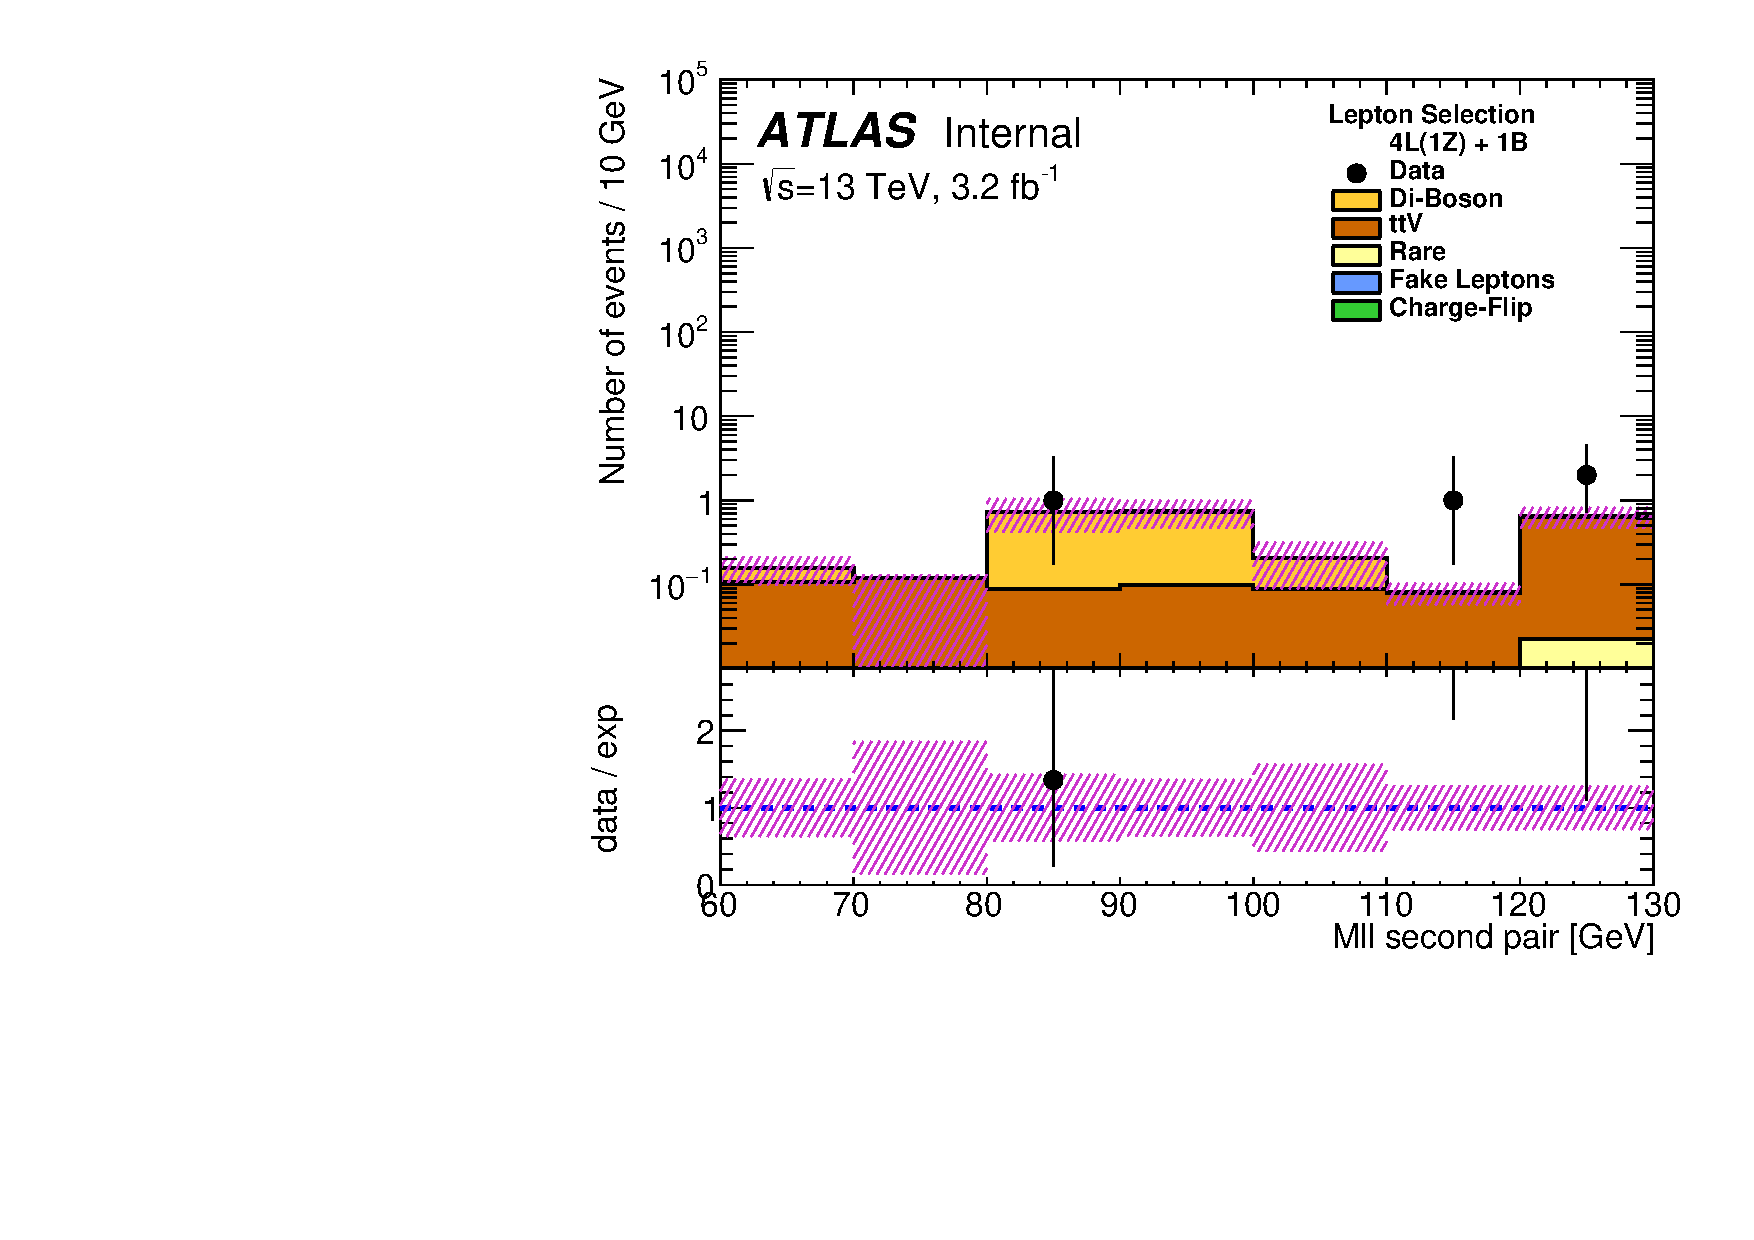
\includegraphics[width=0.5\textwidth]{BKG/validationPLots/TTZ_CR1B4L_MLL2}
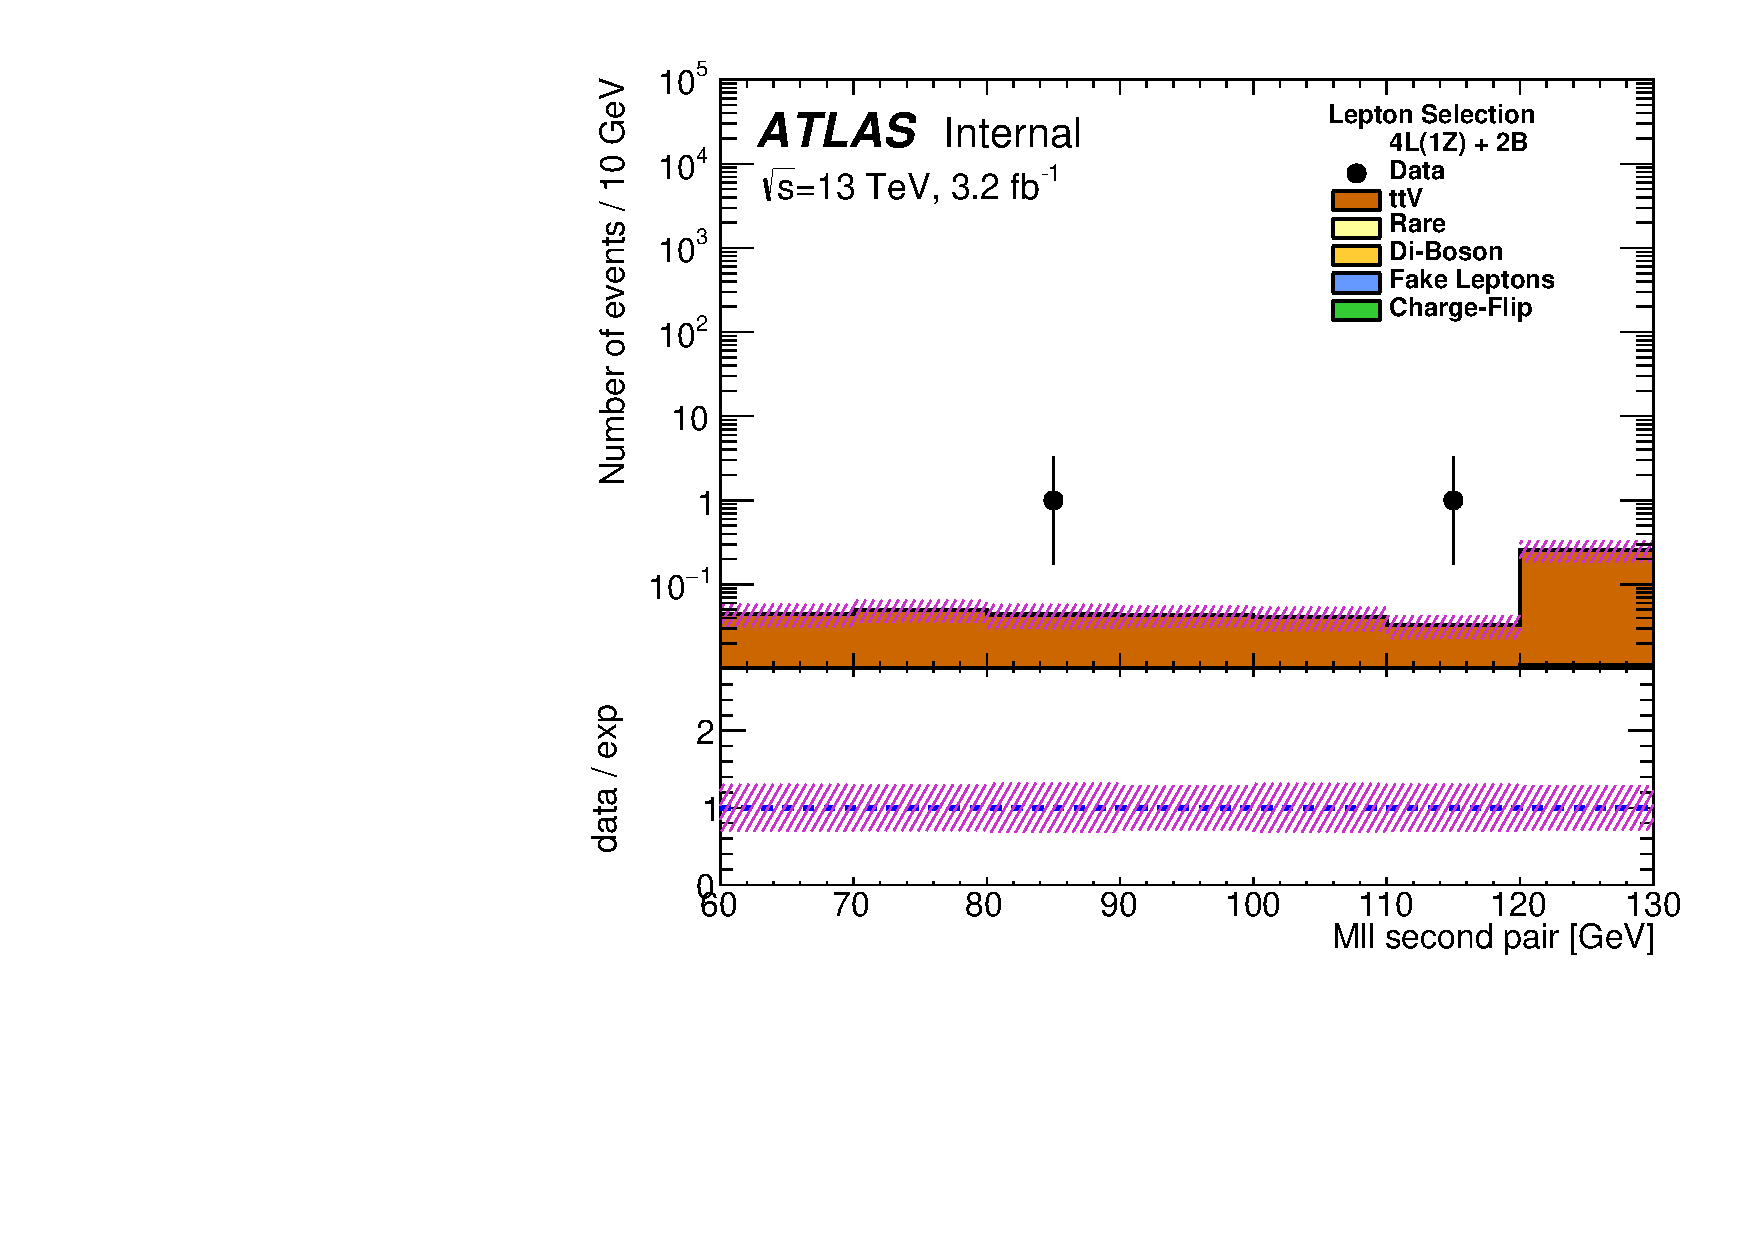
\includegraphics[width=0.5\textwidth]{BKG/validationPLots/TTZ_CR2B4L_MLL2}}
\caption{Distribution of the second $m_{ll}$ pair after requiring at least 1$b$-jet (left) or at least 2$b$-jets (right), and at least four leptons in the event. Note that  there is already one $Z$ boson reconstructed from the other two leptons.}
\label{fig:Results_VR2bttZ_mSecondZ} 
\end{figure} 


\clearpage 
 %%%%%
\par{\bf Results in relaxed \ttbar\ + $Z$ validation regions\\}
In order to see if the observed excess is just a fluctuation we relax the definition of the $ttZ$ 2bIncl region and look at the agreement between the observed number of events and expected background. The obtained results are presented in Table~\ref{tab:ttzr_results} and Table~\ref{tab:ttzr_results_perCh}, with the considered region defined in the upper column of the table. When using a relaxed selection, the obtained results are pointing to a fluctuation in the $ee$ and $e\mu$ channels, whereas, in the $\mu\mu$ channel the tension is still present (even if it is reduced when compared to the nominal selection). 

\begin{table}[htb!]
\caption{Results in relaxed $ttZ$ 2bIncl validation regions. The considered definitions are shown in the upper box of the table. Nominal stands for the $ttZ$ 2bIncl VR as defined in Table~\ref{tab:ttZ_VR}. ``Total'' category includes the number of expected background events.}
\label{tab:ttzr_results}
\begin{center}
\resizebox{0.99\textwidth}{!}{
\begin{tabular}{|c|c|cccccc|} 
\hline\hline
& Nominal& Nominal +                         &  Nominal +  SR, high \met, \meff&  Nominal +                                        &  Nominal +  SR, high \met, \meff     &   Nominal +                                                                                 &  Nominal +  SR, high \met, \meff      \\
&             & $|\eta|_{e1,2}$~$<$~2.& $|\eta|_{e1,2}$~$<$~2.          & $|\eta|_{e1,2}$~$<$~2., no Z cut & $|\eta|_{e1,2}$~$<$~2., no Z cut& $|\eta|_{e1,2}$~$<$~2., no Z cut,  $N_{jets}^{25}$ $\ge$ 3 & $|\eta|_{e1,2}$~$<$~2., no Z cut,  $N_{jets}^{25}$ $\ge$ 3 \\\hline
         Fakes & $-0.25 \pm 0.43 \pm 1.13$ & $-0.25 \pm 0.43 \pm 1.13$ & $0.27 \pm 0.54 \pm 1.54$ & $1.43 \pm 0.77 \pm 3.14$ & $2.37 \pm 0.92 \pm 4.17$ & $2.08 \pm 0.85 \pm 3.93$ & $3.17 \pm 1.00 \pm 5.08$ \\
      ttZ, ttW & $2.60 \pm 0.06 \pm 0.78$ & $2.85 \pm 0.07 \pm 0.86$ & $4.08 \pm 0.08 \pm 1.22$ & $4.11 \pm 0.08 \pm 1.23$ & $6.07 \pm 0.11 \pm 1.82$ & $5.19 \pm 0.10 \pm 1.56$ & $7.36 \pm 0.12 \pm 2.21$ \\\hline
           Total & $3.32 \pm 0.46 \pm 1.65$ & $3.63 \pm 0.46 \pm 1.73$ & $5.62 \pm 0.57 \pm 2.34$ & $7.58 \pm 0.79 \pm 3.81$ & $11.16 \pm 0.95 \pm 5.16$ & $9.82 \pm 0.87 \pm 4.78$ & $13.80 \pm 1.03 \pm 6.27$ \\
           Data & $12 $ & $12  $ & $14  $ & $17 $ & $22 $ & $20 $ & $25  $ \\\hline \hline
          Significance & 2.08  & 1.92  & 1.42  & 1.25 & 1.04  &  1.09 &  0.88  \\ \hline
\end{tabular}} 
\end{center}  
SR, high \met, \meff~=~no cuts ensuring the orthogonality with the SRs and a small BSM contamination.\\
\end{table}
%%
\begin{table}[htb!]
\caption{Results per channel in relaxed $ttZ$ 2bIncl validation regions. The considered definitions are shown in the upper box of the table. Nominal stands for the $ttZ$ 2bIncl VR as defined in Table~\ref{tab:ttZ_VR}. ``Total'' category includes the number of expected background events.}
\label{tab:ttzr_results_perCh}
\begin{center}
\resizebox{0.99\textwidth}{!}{
\begin{tabular}{|c|c|cccccc|} 
\hline\hline
& Nominal& Nominal +                         &  Nominal +  SR, high \met, \meff&  Nominal +                                        &  Nominal +  SR, high \met, \meff     &   Nominal +                                                                                 &  Nominal +  SR, high \met, \meff      \\
&             & $|\eta|_{e1,2}$~$<$~2.& $|\eta|_{e1,2}$~$<$~2.          & $|\eta|_{e1,2}$~$<$~2., no Z cut & $|\eta|_{e1,2}$~$<$~2., no Z cut& $|\eta|_{e1,2}$~$<$~2., no Z cut,  $N_{jets}^{25}$ $\ge$ 3 & $|\eta|_{e1,2}$~$<$~2., no Z cut,  $N_{jets}^{25}$ $\ge$ 3 \\\hline
\hline\multicolumn{8}{c}{\bf $ee$ channel}\\\hline
          Fakes & $-0.42 \pm 0.24 \pm 0.33$ & $-0.42 \pm 0.24 \pm 0.33$ & $-0.26 \pm 0.29 \pm 0.45$ & $0.05 \pm 0.36 \pm 0.68$ & $0.18 \pm 0.39 \pm 0.82$ & $0.21 \pm 0.39 \pm 0.79$ & $0.34 \pm 0.43 \pm 0.94$ \\
      ttZ, ttW & $0.34 \pm 0.02 \pm 0.10$ & $0.42 \pm 0.03 \pm 0.13$ & $0.64 \pm 0.03 \pm 0.19$ & $0.59 \pm 0.03 \pm 0.18$ & $0.95 \pm 0.04 \pm 0.29$ & $0.78 \pm 0.04 \pm 0.23$ & $1.18 \pm 0.05 \pm 0.35$ \\
       Total & $0.05 \pm 0.25 \pm 0.36$ & $0.14 \pm 0.25 \pm 0.38$ & $0.56 \pm 0.29 \pm 0.52$ & $0.99 \pm 0.37 \pm 0.76$ & $1.65 \pm 0.40 \pm 0.97$ & $1.44 \pm 0.40 \pm 0.91$ & $2.15 \pm 0.44 \pm 1.13$ \\
           Data & $3 $ & $3  $ & $3 $ & $3  $ & $3 $ & $3  $ & $3  $ \\\hline
           Significance&0.90 & 1.66 & 1.43&0.92&0.37&0.52&0.05\\
\hline\multicolumn{8}{c}{\bf $e\mu$ channel}\\\hline
          Fakes & $0.09 \pm 0.24 \pm 0.39$ & $0.09 \pm 0.24 \pm 0.39$ & $0.32 \pm 0.35 \pm 0.58$ & $1.23 \pm 0.56 \pm 1.70$ & $1.65 \pm 0.69 \pm 2.33$ & $1.77 \pm 0.65 \pm 2.31$ & $2.34 \pm 0.77 \pm 3.05$ \\
     ttZ, ttW & $1.23 \pm 0.04 \pm 0.37$ & $1.41 \pm 0.05 \pm 0.42$ & $2.03 \pm 0.06 \pm 0.61$ & $1.99 \pm 0.06 \pm 0.60$ & $3.00 \pm 0.07 \pm 0.90$ & $2.53 \pm 0.07 \pm 0.76$ & $3.64 \pm 0.08 \pm 1.09$ \\
        Total & $1.67 \pm 0.25 \pm 0.65$ & $1.89 \pm 0.25 \pm 0.71$ & $2.88 \pm 0.36 \pm 1.01$ & $4.11 \pm 0.57 \pm 1.97$ & $5.84 \pm 0.70 \pm 2.73$ & $5.43 \pm 0.66 \pm 2.63$ & $7.43 \pm 0.79 \pm 3.50$ \\
           Data & $4 $ & $4  $ & $5  $ & $6  $ & $10$ & $7  $ & $11 $ \\\hline
           Significance&0.87&0.71&0.48&0.25&0.61&0.07&0.36\\
\hline\multicolumn{8}{c}{\bf $\mu\mu$ channel}\\\hline
          Fakes & $0.08 \pm 0.27 \pm 0.41$ & $0.08 \pm 0.27 \pm 0.41$ & $0.21 \pm 0.30 \pm 0.51$ & $0.15 \pm 0.37 \pm 0.76$ & $0.54 \pm 0.47 \pm 1.03$ & $0.11 \pm 0.38 \pm 0.83$ & $0.49 \pm 0.47 \pm 1.10$ \\
      ttZ, ttW & $1.02 \pm 0.04 \pm 0.31$ & $1.02 \pm 0.04 \pm 0.31$ & $1.40 \pm 0.05 \pm 0.42$ & $1.53 \pm 0.05 \pm 0.46$ & $2.12 \pm 0.06 \pm 0.64$ & $1.88 \pm 0.06 \pm 0.56$ & $2.54 \pm 0.07 \pm 0.76$ \\
         Total & $1.60 \pm 0.30 \pm 0.67$ & $1.60 \pm 0.30 \pm 0.67$ & $2.18 \pm 0.33 \pm 0.84$ & $2.48 \pm 0.40 \pm 1.12$ & $3.66 \pm 0.50 \pm 1.50$ & $2.95 \pm 0.41 \pm 1.31$ & $4.22 \pm 0.50 \pm 1.71$ \\
           Data & $5  $ & $5  $ & $6$ & $8  $ & $9  $ & $10 $ & $11 $ \\\hline
           Significance&1.33&1.33&1.25&1.65&1.23&1.86&1.42\\\hline
\end{tabular}} 
\end{center}  
SR, high \met, \meff = no cuts ensuring no overlap with the SRs and a small contamination in BSM signal.\\
\end{table}  


 %%%%%
\par{\bf Tightening the signal lepton definition \\}
To decrease the probability of having fake muons in the $ttZ$ 2bIncl region, we further tighten the signal muon definition. First we use muons with ``Tight'' WP instead of ``Medium'' WP, and further we tighten the cut on the track isolation and/or add a cut on the calorimeter isolation. For electrons, as no tighter WP is available, we just tighten the track and the calorimeter isolation requirements. For these results the lepton fake rate is not remeasured (i.e the nominal fake rate is used). The results are shown in Tables~\ref{table:Yields_MediumMu} and~\ref{table:Yields_TightMu}. Generally it observed that the excess is reduced when considering tighter isolation criteria (i.e a cut value of 0.01 and adding a cut on the calorimeter isolation for muons). 

\begin{sidewaystable}[ph!]
\centering
\renewcommand{\arraystretch}{1.2}
{
\resizebox{1.\textwidth}{!}{
\begin{tabular}{|c|c|c|c|c|c|c|} \hline
& Nominal  & $e$ nominal                               & $e$ nominal                                  & $e$ nominal                                               & $e$ track + calo iso $<$ 0.01*\pt   & $e$ track + calo iso $<$ 0.01*\pt   \\
&               & $\mu$ calo iso $<$ 0.06*\pt    & $\mu$ track iso $<$ 0.01*\pt      & $\mu$ track + calo iso $<$ 0.01*\pt         & $\mu$ nominal                                  & $\mu$ track iso $<$ 0.01*\pt           \\\hline 
Fakes & $-0.25 \pm 0.43 \pm 1.13$& $-0.30 \pm 0.37 \pm 1.00$ & $-0.33 \pm 0.37 \pm 1.03$ & $0.10 \pm 0.41 \pm 1.04$ & $0.30 \pm 0.46 \pm 1.18$ & $0.22 \pm 0.41 \pm 1.08$ \\
 ttZ, ttW  & $2.60 \pm 0.06 \pm 0.78$ & $2.36 \pm 0.06 \pm 0.71$ & $2.36 \pm 0.06 \pm 0.71$ & $1.54 \pm 0.05 \pm 0.46$& $1.86 \pm 0.05 \pm 0.56$& $1.46 \pm 0.05 \pm 0.44$\\
ttH & $0.15 \pm 0.04 \pm 0.07$& $0.13 \pm 0.04 \pm 0.06$& $0.13 \pm 0.04 \pm 0.07$& $0.07 \pm 0.04 \pm 0.04$& $0.11 \pm 0.04 \pm 0.05$ & $0.09 \pm 0.04 \pm 0.04$ \\
Di-Boson & $0.31 \pm 0.13 \pm 0.09$ & $0.31 \pm 0.13 \pm 0.09$ & $0.29 \pm 0.13 \pm 0.09$ & $0.29 \pm 0.13 \pm 0.09$& $0.22 \pm 0.12 \pm 0.07$ & $0.17 \pm 0.12 \pm 0.05$\\
Rare  & $0.52 \pm 0.06 \pm 0.26$ & $0.44 \pm 0.06 \pm 0.22$& $0.46 \pm 0.06 \pm 0.23$  & $0.28 \pm 0.04 \pm 0.14$ & $0.37 \pm 0.05 \pm 0.19$ & $0.23 \pm 0.04 \pm 0.11$\\\hline
Total  & $3.33 \pm 0.46 \pm 1.66$& $2.94 \pm 0.40 \pm 1.47$ & $2.91 \pm 0.41 \pm 1.50$ & $2.27 \pm 0.44 \pm 1.26$ & $2.86 \pm 0.48 \pm 1.46$& $2.17 \pm 0.43 \pm 1.26$\\
Data & $12 $  & 10 &11& 7 &9&8\\ \hline\hline
Significance & 2.08 & 1.87&2.21 &1.48 &1.65&1.85\\ \hline
\end{tabular}}
\caption{Results in relaxed $ttZ$ 2bIncl validation regions. The changes in the signal lepton definition are shown in the upper box of the table; the electron isolation is changed only if \pt$_e < 300$~\GeV. Nominal stands for the $ttZ$ 2bIncl VR as defined in Table~\ref{tab:ttZ_VR}. ``Total'' category includes the number of expected background events.}
\label{table:Yields_MediumMu}
}

{
\resizebox{1.\textwidth}{!}{
\begin{tabular}{|c|c|c|c|c|c|c|} \hline
 &$e$ nominal         & $e$ nominal                               & $e$ nominal                                  & $e$ nominal                                               & $e$ track + calo iso $<$ 0.01*\pt   & $e$ track + calo iso $<$ 0.01*\pt       \\
 &$\mu_T$ nominal & $\mu_T$ calo iso $<$ 0.06*\pt & $\mu_T$ track iso $<$ 0.01*\pt  & $\mu_T$ track + calo iso $<$ 0.01*\pt    & $\mu_T$ nominal                               & $\mu_T$ track iso $<$ 0.01*\pt           \\\hline 
Fakes &  $-0.25 \pm 0.43 \pm 1.13$ & $-0.30 \pm 0.37 \pm 1.00$& $-0.33 \pm 0.37 \pm 1.03$ & $0.10 \pm 0.41 \pm 1.04$ & $0.30 \pm 0.46 \pm 1.18$& $0.22 \pm 0.41 \pm 1.08$ \\
 ttZ, ttW  & $2.36 \pm 0.06 \pm 0.71$ & $2.15 \pm 0.06 \pm 0.64$& $2.14 \pm 0.06 \pm 0.64$& $1.41 \pm 0.05 \pm 0.42$& $1.65 \pm 0.05 \pm 0.49$& $1.46 \pm 0.05 \pm 0.44$\\
ttH & $0.14 \pm 0.04 \pm 0.07$  & $0.11 \pm 0.04 \pm 0.06$& $0.12 \pm 0.04 \pm 0.06$& $0.06 \pm 0.03 \pm 0.03$& $0.10 \pm 0.04 \pm 0.05$ & $0.09 \pm 0.04 \pm 0.04$\\
Di-Boson &  $0.29 \pm 0.13 \pm 0.09$& $0.28 \pm 0.13 \pm 0.08$ & $0.26 \pm 0.13 \pm 0.08$& $0.26 \pm 0.13 \pm 0.08$ & $0.20 \pm 0.12 \pm 0.06$ & $0.17 \pm 0.12 \pm 0.05$\\
Rare  &  $0.40 \pm 0.05 \pm 0.20$& $0.33 \pm 0.05 \pm 0.16$ & $0.36 \pm 0.05 \pm 0.18$ & $0.22 \pm 0.04 \pm 0.11$ & $0.26 \pm 0.04 \pm 0.13$ & $0.23 \pm 0.04 \pm 0.11$\\\hline
Total  &  $2.92 \pm 0.46 \pm 1.55$ & $2.57 \pm 0.40 \pm 1.38$ & $2.55 \pm 0.40 \pm 1.41$ & $2.05 \pm 0.43 \pm 1.22$  & $2.50 \pm 0.48 \pm 1.39$& $2.17 \pm 0.43 \pm 1.26$ \\
Data &  $12$ &10 & 11 & 7 & 9 &8\\ \hline\hline
Significance & 2.32 & 2.11 &2.36&1.63 & 1.88&1.85\\ \hline
\end{tabular}}
\caption{Results in relaxed $ttZ$ 2bIncl validation regions. The changes in the signal lepton definition are shown in the upper box of the table; $\mu_T$ stands for muons passing \texttt{Tight} WP instead of \texttt{Medium} as used in this analysis; the electron isolation is changed only if \pt$_e < 300$~\GeV. Nominal stands for the $ttZ$ 2bIncl VR as defined in Table~\ref{tab:ttZ_VR}. ``Total'' category includes the number of expected background events.}
\label{table:Yields_TightMu}
}

\end{sidewaystable}
 
 
 %%%%%
\par{\bf Conclusions \\}
Given all the performed cross-checks no obvious problem is found, and the tension observed in the $ttZ$ 1bIncl region tends to be just a fluctuation. However, it will be very interesting to study the region with at least two $b$-jets and low \meff\ when more data will be available.
